\section*{Test 4 Measurement of the fundamental diagram}

The figure shown below (Figure 3) is to be modelled (corridor 1000 m long, 10 m wide). There are three measuring points (2 x 2 m), the dotted of which is the main measuring point, with the other two grey measuring points functioning as control measuring points.

\noindent
The corridor is to be filled with different densities of persons with an equal as possible free walking speed (for example 1.2 – 1.4m/s): 0.5 P/m $^2$, 1 P/m$^2$, 2 P/m$^2$, 3 P/m$^2$, 4 P/m$^2$, 5 P/m$^2$ and 6 P/m$^2$.

\noindent
At the measuring points, the average speed of persons over a period of 60 seconds is to be determined for the specified density. The first 10 seconds can be ignored as a "transient response". From the results (speed at the specified density), the corresponding fundamental diagrams can be created, with the calculation flow = speed * density taken as a basis for the flow of persons.
 
\noindent
In order to ensure that the fundamental diagram is also reproduced by the program in case of a "line movement", the corridor should be reduced in width to such a degree that the persons can only move one behind the other and overtaking is not possible.




\begin{figure}[h]
	\centering
	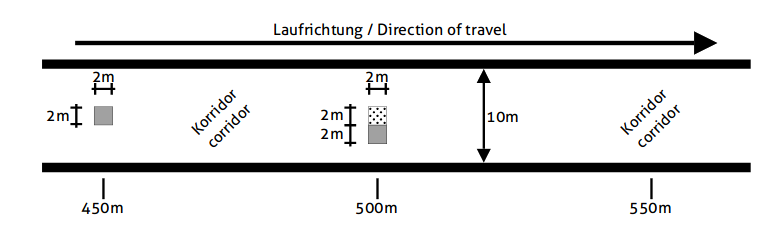
\includegraphics[scale=0.50]{test_description/Corridor_tets_4.png}
	\caption{\footnotesize \textbf{Measurement of the fundamental diagram}}
\end{figure}


